\chapter{Performance results for self-optimizing cloud} % Write in your own chapter title
\label{Chapter_performance}
\lhead{Chapter \ref{Chapter_performance}. \emph{Performance results for self-optimizing cloud}} % Write in your own chapter title to set the page header

\section{Test-bed Autonomic Computing Performance Tests}

This section will present the performance of the self-organizing, self-optimizing autonomic system presented in this thesis when run on top of the test bed under various loads. The goal of this section is to determine how the system behaves when being overloaded or underloaded.

The tests are split such that the same scenario is tested with various numbers of starting servers in the cluster and various loads such that up scaling, down scaling and no scaling are all tested. The tests are run slightly longer than 30 minutes, due to the fact that there is a ramp up at the beginning of the test while clients join, sessions are created and clients start streaming.

\subsection{Single server start}

The first set of tests starts with a single server in the cloud. In this case, if the cloud is underloaded the server will not be removed from the cloud as that will leave no servers servicing user requests.

\subsubsection{Under-load cloud}

This test case tests the base case of an under-loaded cloud, where the cloud contains a single server and the number of clients and streams can be easily handled by the single server.

Figure \ref{fig:1serv-ant} shows the pheromone level as seen by the ant. The top and bottom dotted red lines represent the thresholds for adding/removing servers to/from the cloud. The middle dotted blue line represents the starting pheromone level. When the pheromone passes the higher threshold servers are removed and when the pheromone passes the lower threshold servers are added to the cloud. Once the threshold is passed the ant goes to the manager which attempts to optimize the cloud's server count - this can be observed at the top of the graph where it plateaus as that is time when the ant is at the manager. In this case the optimization will result in no change as this is the only server in the cloud and it can not be removed. After optimization the ant returns to the server and restarts the process from the base state of the system. Figure \ref{fig:1serv-pher} shows the pheromone as seen at the server. Since there is one server and one ant the values are very close, however in the server figure the pheromone decay can also be observed. 

Finally, figure \ref{fig:1serv-perf} shows the performance of the server. The optimization of the system starts at the same time the first stream begins seen on the bandwidth graph when the bandwidth value goes up. In this case it can be seen that the CPU is barely used and also latencies are low and bandwidth is not high, as such the system wishes to remove servers from the cloud.

\begin{figure}
	\centering
		\includegraphics[width=0.95\columnwidth]{results/Run-1-low/ant-1.png}
	\caption{Under-loaded cloud - Pheromone as seen by Ant 1}
	\label{fig:1serv-ant}
\end{figure}

\begin{figure}
	\centering
		\includegraphics[width=0.95\columnwidth]{results/Run-1-low/server-1.png}
	\caption{Under-loaded cloud - Pheromone as seen by Server 1}
	\label{fig:1serv-pher}
\end{figure}

\begin{figure}
	\centering
		\includegraphics[width=0.95\columnwidth]{results/Run-1-low/perf-1.png}
	\caption{Under-loaded cloud - Server 1 performance}
	\label{fig:1serv-perf}
\end{figure}

\subsubsection{Medium/low loaded cloud}

In this test case the cloud is still underloaded but the load is closer to what a single server can support. As such it can be seen that in figure \ref{fig:1serv-ant-lowmed} the pheromone level increases slower than in figure \ref{fig:1serv-ant} and similarly for figures \ref{fig:1serv-pher-lowmed} and figure \ref{fig:1serv-pher-lowmed}. At the same time figure  \ref{fig:1serv-perf-lowmed} shows that the CPU usage is higher than in the previous test case, while bandwidth usage and latencies are also higher.

\begin{figure}[!ht]
	\centering
		\includegraphics[width=0.95\columnwidth]{results/Run-1-lowmed/ant-1.png}
	\caption{Medium/low loaded cloud - Pheromone as seen by Ant 1}
	\label{fig:1serv-ant-lowmed}
\end{figure}

\begin{figure}
	\centering
		\includegraphics[width=0.95\columnwidth]{results/Run-1-lowmed/server-1.png}
	\caption{Medium/low loaded cloud - Pheromone as seen by Server 1}
	\label{fig:1serv-pher-lowmed}
\end{figure}

\begin{figure}
	\centering
		\includegraphics[width=0.95\columnwidth]{results/Run-1-lowmed/perf-1.png}
	\caption{Medium/low loaded cloud - Server 1 performance}
	\label{fig:1serv-perf-lowmed}
\end{figure}

\subsubsection{Medium loaded cloud}

This test case tests a server which is neither overloaded nor underloaded. As such, the pheromone level should stay stable such that servers are not added or removed from the cloud. As seen in graphs \ref{fig:1serv-ant-med} and \ref{fig:1serv-pher-med} the pheromone level is largely stable except for two spikes around 14 and 29 minutes in. The two spikes coincide with the streams stopping and in figure \ref{fig:1serv-perf-med} it can be noticed that at those times the CPU usage and latency drops down, resulting in the server being underloaded for a brief period of time.

\begin{figure}[!ht]
	\centering
		\includegraphics[width=0.95\columnwidth]{results/Run-1-med/ant-1.png}
	\caption{Medium loaded cloud - Pheromone as seen by Ant 1}
	\label{fig:1serv-ant-med}
\end{figure}

\begin{figure}
	\centering
		\includegraphics[width=0.95\columnwidth]{results/Run-1-med/server-1.png}
	\caption{Medium loaded cloud - Pheromone as seen by Server 1}
	\label{fig:1serv-pher-med}
\end{figure}

\begin{figure}
	\centering
		\includegraphics[width=0.95\columnwidth]{results/Run-1-med/perf-1.png}
	\caption{Medium loaded cloud - Server 1 performance}
	\label{fig:1serv-perf-med}
\end{figure}

\subsubsection{Medium/high loaded cloud}

In this test case the cloud is overloaded but barely above what a single server can accommodate. Looking at graph \ref{fig:1serv-pher-medhigh} it can be noticed that the pheromone level drops for the first 12 - 13 minutes after which a second server is added, which can be noticed by the second server appearing on the graph.  Because two servers are two much for this load the pheromone level increases until the thresholds are breached again and one of the servers is stopped. Figure \ref{fig:1serv-pher-medhigh} shows the pheromone at the two servers and matches what the ants see as well.

The performance graphs show high bandwidth and high CPU usage until the second server is added, at which time the cloud is rebalanced and the bandwdith and CPU are lower for each of the two servers. Average latency for the clients also drops when the second server is added.

\begin{figure}
	\centering
		\includegraphics[width=0.95\columnwidth]{results/Run-1-medhigh/server-1.png}
	\caption{Medium/high loaded cloud - Pheromone as seen by servers}
	\label{fig:1serv-pher-medhigh}
\end{figure}

\begin{figure}
	\centering
		\includegraphics[width=0.95\columnwidth]{results/Run-1-medhigh/perf-1.png}
	\caption{Medium/high loaded cloud - Server performance}
	\label{fig:1serv-perf-medhigh}
\end{figure}

In terms of optimization by the house hunting algorithm the up scaling of the cloud is trivial as there is a single ant so there is no recruitment needed. When the cloud is down scaled however the house hunting algorithm runs. In the first round each of the two ants chooses a new server count - in this case both choose to remove one server and then they simulate the solution. One ant's solution fitness is 0.519 while the other ant's is 0.497. The ants then go through recruitment and the ant with fitness 0.497 recruits the other ant to it's nest. Because all ants at this point go to the same nest, this is the solution of the optimization and one of the servers is removed.

\subsubsection{Over-loaded cloud}

This test is set up such that a single server can not handle by itself the requests sent by clients, and as such it is expected that a second server will be added to the cloud and not be removed. This can be seen in figure \ref{fig:1serv-pher-high} as the pheromone level drops initially very fast until a second server is added. After the second server is added the pheromone level increases for some time but stabilizes after that. While server two has a pheromone level higher than the upper threshold, the average pheromone across the cloud is bellow the thresholds. 

The performance graphs show high CPU, bandwidth and latency before the second server is added. After the second server is added the performance metrics stabilize at good values. The optimization by the house hunting algorithm is also trivial as there is a single ant to begin with, so no recruitment can happen.

\begin{figure}
	\centering
		\includegraphics[width=0.95\columnwidth]{results/Run-1-high/server-1.png}
	\caption{Over-loaded cloud - Pheromone as seen by servers}
	\label{fig:1serv-pher-high}
\end{figure}

\begin{figure}
	\centering
		\includegraphics[width=0.95\columnwidth]{results/Run-1-high/perf-1.png}
	\caption{Over-loaded cloud - Server performance}
	\label{fig:1serv-perf-high}
\end{figure}

\subsection{Two server start}

This set of tests start with two servers in the cloud and different loads.

\subsubsection{Under-load cloud}

This test case tests the base case of an under-loaded cloud, where the cloud starts with two servers but the number of clients and streams can be easily handled by a single server. Figure \ref{fig:2serv-pher-low} shows the pheromone level from the server's perspective. The pheromone goes up at both servers and after the threshold is reached one of the two servers is removed. After the removal the load is still too low for the single server and the pheromone level continues increasing. 

The server performance graphs show that the servers are under-loaded and even after the server is removed the load on the single remaining server is low enough not to cause a breach of SLA.

\begin{figure}
	\centering
		\includegraphics[width=0.75\columnwidth]{results/Run-2-low/server-1.png}
	\caption{Under-loaded cloud - Pheromone as seen by servers}
	\label{fig:2serv-pher-low}
\end{figure}

\begin{figure}
	\centering
		\includegraphics[width=0.75\columnwidth]{results/Run-2-low/perf-1.png}
	\caption{Under-loaded cloud - Server performance}
	\label{fig:2serv-perf-low}
\end{figure}

\subsubsection{Medium/low loaded cloud}

Similarly to the previous test, this test does not generate enough load for both servers. Unlike the previous test, which has a very low load, the load in this test is closer to the load of a well balanced cloud. Figure \ref{fig:2serv-pher-medlow} shows the pheromone as seen by the server. The pheromone increases similar to the previous test but at a lower rate. As before, the load is quite low on the two servers and once one of the two servers is removed the other server can take the load without problems.

\begin{figure}
	\centering
		\includegraphics[width=0.75\columnwidth]{results/Run-2-lowmed/server-1.png}
	\caption{Medium/low loaded cloud - Pheromone as seen by servers}
	\label{fig:2serv-pher-medlow}
\end{figure}

\begin{figure}
	\centering
		\includegraphics[width=0.75\columnwidth]{results/Run-2-lowmed/perf-1.png}
	\caption{Medium/low loaded cloud - Server performance}
	\label{fig:2serv-perf-medlow}
\end{figure}

\subsubsection{Medium loaded cloud}

This test case puts enough load on the cloud to require two servers to provide good QoS to the clients. Figure \ref{fig:2serv-pher-med} shows the pheromone levels as seen at the servers. Looking at the performance graphs in figure \ref{fig:2serv-perf-med} it can be noticed that the two servers are not perfectly balanced as server 2 has a lower load than server 1 as seen by CPU utilization, bandwidth and latency. As such, the pheromone level at server 2 increases while the pheromone level at server 1 stays stable. Even though one server has increasing pheromone values no servers are removed because the ants history has a lower average pheromone than the threshold.

\begin{figure}
	\centering
		\includegraphics[width=0.75\columnwidth]{results/Run-2-med/server-1.png}
	\caption{Medium loaded cloud - Pheromone as seen by servers}
	\label{fig:2serv-pher-med}
\end{figure}

\begin{figure}
	\centering
		\includegraphics[width=0.75\columnwidth]{results/Run-2-med/perf-1.png}
	\caption{Medium loaded cloud - Server performance}
	\label{fig:2serv-perf-med}
\end{figure}

\subsubsection{Medium/high loaded cloud}

In this test the load is higher than what two servers can support but not by a significant amount. Initially in figure \ref{fig:2serv-pher-medhigh} the pheromone level drops at the beginning of the test. After the threshold is breached one new server is added. After the server is added the system is largely stable, however due to the servers not being balanced server 1 sees an increase in pheromone levels. This increase however is not enough to cause a SLA breach as the other two servers are within proper bounds.

Performance graphs show that the two servers are overloaded in the beginning and after the addition of the new servers, the system becomes stable until the end of the test.

\begin{figure}
	\centering
		\includegraphics[width=0.75\columnwidth]{results/Run-2-medhigh/server-1.png}
	\caption{Medium/high loaded cloud - Pheromone as seen by servers}
	\label{fig:2serv-pher-medhigh}
\end{figure}

\begin{figure}
	\centering
		\includegraphics[width=0.75\columnwidth]{results/Run-2-medhigh/perf-1.png}
	\caption{Medium/high loaded cloud - Server performance}
	\label{fig:2serv-perf-medhigh}
\end{figure}

\subsubsection{Over loaded cloud}

Finally a test was run where the cloud is overloaded significantly for two servers. This can be seen in figure \ref{fig:2serv-pher-high} as the pheromone level drops at the beginning of the test. After the threshold is breached two new servers are added. Because after the two servers are added the cloud is not well balanced server 1 sees an increase in pheromone, while servers 3 and 4 see a decrease with server 2 being stable. Once server 1 stabilizes however, there are too many servers in the cloud due to the fact that the clients stop streaming. As such the servers are removed until one server remains in the cloud.

Performance graphs show that the two servers are overloaded in the beginning and after the addition of the two new servers, the system becomes stable until the end of the test.

\begin{figure}
	\centering
		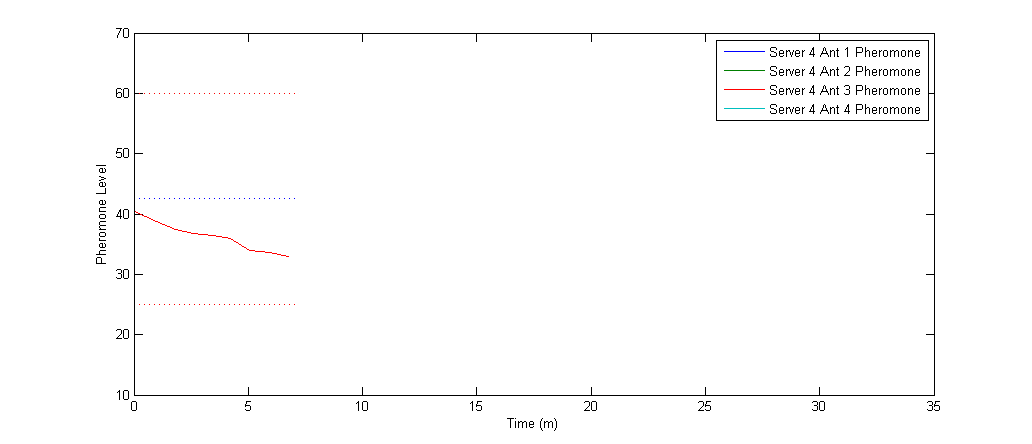
\includegraphics[width=0.75\columnwidth]{results/Run-2-high/ant-13.png}
	\caption{Over-loaded cloud - Pheromone at Server 4 as seen by ants}
	\label{fig:2serv-ant13-high}
\end{figure}

\begin{figure}
	\centering
		\includegraphics[width=0.75\columnwidth]{results/Run-2-high/server-1.png}
	\caption{Over-loaded cloud - Pheromone as seen by servers}
	\label{fig:2serv-pher-high}
\end{figure}

\begin{figure}
	\centering
		\includegraphics[width=0.75\columnwidth]{results/Run-2-high/perf-1.png}
	\caption{Over-loaded cloud - Server performance}
	\label{fig:2serv-perf-high}
\end{figure}

\subsection{Three server start}

This set of tests start with three servers in the cloud and different loads.

\subsubsection{Under loaded cloud}

Similar to the other cases the first test is started with a load which a single server can easily meet. As seen in figure \ref{fig:3serv-pher-low} the pheromone level increases, and one of the server is removed. After the removal the pheromone level continues to increase but slower since a single server is sufficient. After the threshold is reached again a second server is removed and the cloud stabilizes. The performance graphs show that the load is taken by the other remaining server without any problems.

For the house hunting optimization once the ants simulate the solutions, the initial state is that two of the ants want to remove 2 servers while one of the ants wishes to remove a single server.

\begin{enumerate}
	\item Initial solutions: 
	\begin{itemize}
		\item Ant 1 goes to Nest 1 - remove one servers
		\item Ant 2 goes to Nest 2 - remove two servers
		\item Ant 3 goes to Nest 3 - remove two server
	\end{itemize}
	\item Recruitment:
	\begin{itemize}
		\item Ant 1 recruits Ant 2 and nest 2 is dropped out as no ants go to it
		\item Ant 3 recruits a newly created ant which looks like Ant 3
	\end{itemize}
	\item Recruitment:
	\begin{itemize}
		\item Ant 1 recruits Ant 4
		\item Ant 2 recruits Ant 3
	\end{itemize}
	\item All ants go to same solution which is nest 1
\end{enumerate}

\begin{figure}
	\centering
		\includegraphics[width=0.75\columnwidth]{results/Run-3-low/server-1.png}
	\caption{Under loaded cloud - Pheromone as seen by servers}
	\label{fig:3serv-pher-low}
\end{figure}

\begin{figure}
	\centering
		\includegraphics[width=0.75\columnwidth]{results/Run-3-low/perf-1.png}
	\caption{Under loaded cloud - Server performance}
	\label{fig:3serv-perf-low}
\end{figure}

\subsubsection{Medium/low loaded cloud}

In the medium/low scenario the pheromone level increases slower than in the underloaded scenario as one server is sufficient for the workload, but it would put more strain on a single server as seen in figure \ref{fig:3serv-perf-lowmed}. In this case, once the threshold is reached, the house hunting optimization chooses to remove two servers. The initial solution set all choose to remove two servers, however the system still goes through the house hunting optimization algorithm.

\begin{enumerate}
	\item Initial solutions: 
	\begin{itemize}
		\item Ant 1 goes to Nest 1 - remove two servers
		\item Ant 2 goes to Nest 2 - remove two servers
		\item Ant 3 goes to Nest 3 - remove two servers
	\end{itemize}
	\item Recruitment:
	\begin{itemize}
		\item Ant 2 recruits Ant 1 and nest 1 is dropped out as no ants go to it
		\item Ant 3 recruits a newly created ant which looks like Ant 3
	\end{itemize}
	\item Recruitment:
	\begin{itemize}
		\item Ant 2 recruits Ant 3
		\item Ant 1 recruits Ant 4
	\end{itemize}
	\item All ants go to same solution which is nest 2
\end{enumerate}

\begin{figure}
	\centering
		\includegraphics[width=0.75\columnwidth]{results/Run-3-lowmed/server-1.png}
	\caption{Medium/low loaded cloud - Pheromone as seen by servers}
	\label{fig:3serv-pher-lowmed}
\end{figure}

\begin{figure}
	\centering
		\includegraphics[width=0.75\columnwidth]{results/Run-3-lowmed/perf-1.png}
	\caption{Medium/low loaded cloud - Server performance}
	\label{fig:3serv-perf-lowmed}
\end{figure}

\subsubsection{Medium loaded cloud}

In the well balanced cloud case, one of the servers has less load than the other two servers and as such it has less bandwidth used when compared to the other two servers as seen in figure \ref{fig:3serv-perf-lowmed} - server 3 has less load. Because of this the pheromone at server 3 increases while the pheromone at the other two servers decreases. However, the average pheromone level across the cloud as seen by the ants is always bellow the thresholds and no house hunting optimization is triggered.

\begin{figure}
	\centering
		\includegraphics[width=0.75\columnwidth]{results/Run-3-med/ant-1.png}
	\caption{Medium loaded cloud - Pheromone at Server 1 as seen by ants}
	\label{fig:3serv-ant1-med}
\end{figure}

\begin{figure}
	\centering
		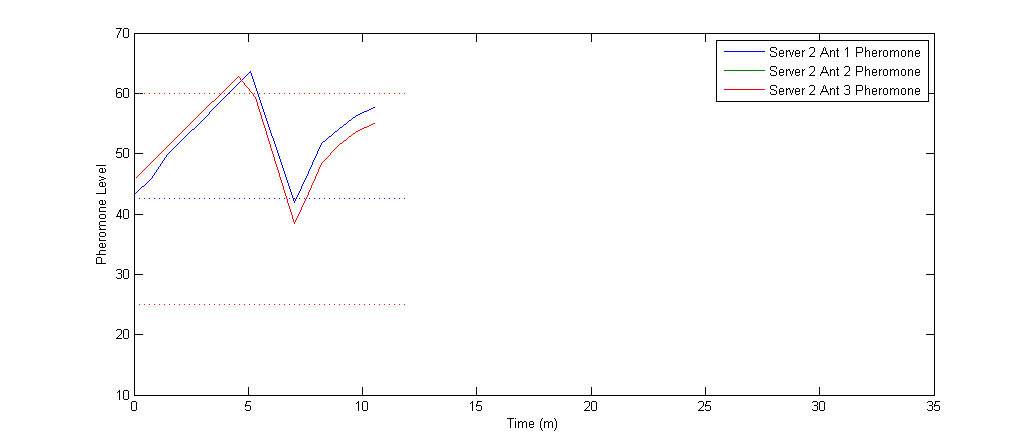
\includegraphics[width=0.75\columnwidth]{results/Run-3-med/ant-4.png}
	\caption{Medium loaded cloud - Pheromone at Server 2 as seen by ants}
	\label{fig:3serv-ant4-med}
\end{figure}

\begin{figure}
	\centering
		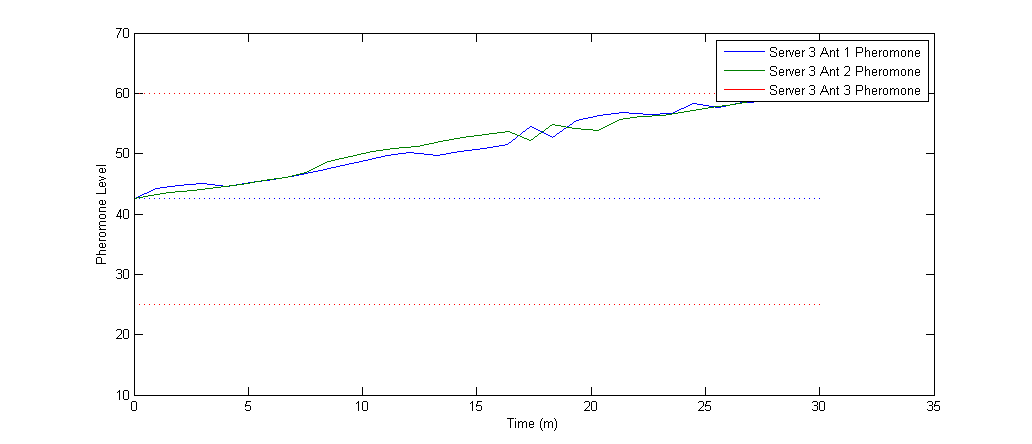
\includegraphics[width=0.75\columnwidth]{results/Run-3-med/ant-7.png}
	\caption{Medium loaded cloud - Pheromone at Server 3 as seen by ants}
	\label{fig:3serv-ant7-med}
\end{figure}

\begin{figure}
	\centering
		\includegraphics[width=0.75\columnwidth]{results/Run-3-med/server-1.png}
	\caption{Medium loaded cloud - Pheromone as seen by servers}
	\label{fig:3serv-pher-med}
\end{figure}

\begin{figure}
	\centering
		\includegraphics[width=0.75\columnwidth]{results/Run-3-med/perf-1.png}
	\caption{Medium loaded cloud - Server performance}
	\label{fig:3serv-perf-med}
\end{figure}

\subsubsection{Medium/high loaded cloud}

This test case tests a cloud which is slightly overloaded. The three servers are insufficient to meet the demands of the clients but barely, as can be seen in figure \ref{fig:3serv-perf-medhigh} where the CPU usage, bandwidth and latency show that more servers are needed to serve clients in the cloud. After approximately 12 minutes an SLA breach is detected and the house hunting optimization algorithm runs and decides to add 2 more servers to the cloud. After the two new servers are added one of the servers is underloaded, two of the servers are properly loaded and two of the servers are overloaded, as seen in figure \ref{fig:3serv-pher-medhigh} where after 15 minutes Server 2 and Server 5 maintain good pheromone levels, Server 1 has increasing pheromone levels (thus being underloaded) while servers 3 and 4 have decreasing pheromones being overloaded. This can also be seen in figure \ref{fig:3serv-perf-medhigh} looking at the bandwidth up graphs, where server 1 has very low bandwidth used, servers 3 and 4 have high bandwidth and servers 2 and 5 have medium bandwidth used.

\begin{figure}
	\centering
		\includegraphics[width=0.75\columnwidth]{results/Run-3-medhigh/ant-1.png}
	\caption{Medium/high loaded cloud - Pheromone at Server 1 as seen by ants}
	\label{fig:3serv-ant1-medhigh}
\end{figure}

\begin{figure}
	\centering
		\includegraphics[width=0.75\columnwidth]{results/Run-3-medhigh/ant-6.png}
	\caption{Medium/high loaded cloud - Pheromone at Server 2 as seen by ants}
	\label{fig:3serv-ant6-medhigh}
\end{figure}

\begin{figure}
	\centering
		\includegraphics[width=0.75\columnwidth]{results/Run-3-medhigh/ant-11.png}
	\caption{Medium/high loaded cloud - Pheromone at Server 3 as seen by ants}
	\label{fig:3serv-ant11-medhigh}
\end{figure}

\begin{figure}
	\centering
		\includegraphics[width=0.75\columnwidth]{results/Run-3-medhigh/ant-16.png}
	\caption{Medium/high loaded cloud - Pheromone at Server 4 as seen by ants}
	\label{fig:3serv-ant16-medhigh}
\end{figure}

\begin{figure}
	\centering
		\includegraphics[width=0.75\columnwidth]{results/Run-3-medhigh/ant-21.png}
	\caption{Medium/high loaded cloud - Pheromone at Server 5 as seen by ants}
	\label{fig:3serv-ant25-medhigh}
\end{figure}

\begin{figure}
	\centering
		\includegraphics[width=0.75\columnwidth]{results/Run-3-medhigh/server-1.png}
	\caption{Medium/high loaded cloud - Pheromone as seen by servers}
	\label{fig:3serv-pher-medhigh}
\end{figure}

\begin{figure}
	\centering
		\includegraphics[width=0.75\columnwidth]{results/Run-3-medhigh/perf-1.png}
	\caption{Medium/high loaded cloud - Server performance}
	\label{fig:3serv-perf-medhigh}
\end{figure}

\subsubsection{Over loaded/under loaded cloud}

In this case the cloud is first over loaded and then suddenly the streaming clients stop and the cloud becomes underloaded. In the first part of the test the three servers are insufficient to meet the demands of the clients as seen in the performance graphs with high bandwidth, latency and CPU usage. This causes the pheromone in the cloud to drop until a SLA breach is detected and new servers are added to the cloud. The pheromone drop is faster than in the previous case due to more load on the server. After new servers are added to the cloud the performance improves as seen by lower bandwidth at each servers, and this remains stable until users stop streaming, at which point the usage drops and the pheromone increases until a new SLA breach is detected and three servers are removed.

The first SLA breach results in two servers being added to the cloud. This is because of the fact that all three ants' initial solution starts with adding 2 new servers. The second SLA breach is more interesting however:

\begin{enumerate}
	\item Initial solutions: 
	\begin{itemize}
		\item Ant 1 goes to Nest 1 - remove three servers
		\item Ant 2 goes to Nest 2 - remove two servers
		\item Ant 3 goes to Nest 3 - remove four server
		\item Ant 4 goes to Nest 4 - remove three server
		\item Ant 5 goes to Nest 5 - remove three server
	\end{itemize}
	\item Recruitment:
	\begin{itemize}
		\item Ant 1 recruits Ant 4 and nest 4 is dropped out as no ants go to it
		\item Ant 5 recruits Ant 3 and nest 3 is dropped out as no ants go to it
		\item Ant 2 recruits a newly created ant which looks like Ant 2
	\end{itemize}
	\item Recruitment:
	\begin{itemize}
		\item Ant 1 recruits Ant 5 and Ant 4 recruits ant 3, nest 5 is dropped out
	\end{itemize}
	\item Recruitment:
	\begin{itemize}
		\item Ant 1 recruits Ant 2
	\end{itemize}
	\item All ants go to same solution which is nest 1
\end{enumerate}

\begin{figure}
	\centering
		\includegraphics[width=0.75\columnwidth]{results/Run-3-high/ant-1.png}
	\caption{Over loaded cloud - Pheromone at Server 1 as seen by ants}
	\label{fig:3serv-ant1-high}
\end{figure}

\begin{figure}
	\centering
		\includegraphics[width=0.75\columnwidth]{results/Run-3-high/ant-6.png}
	\caption{Over loaded cloud - Pheromone at Server 2 as seen by ants}
	\label{fig:3serv-ant6-high}
\end{figure}

\begin{figure}
	\centering
		\includegraphics[width=0.75\columnwidth]{results/Run-3-high/ant-11.png}
	\caption{Over loaded cloud - Pheromone at Server 3 as seen by ants}
	\label{fig:3serv-ant11-high}
\end{figure}

\begin{figure}
	\centering
		\includegraphics[width=0.75\columnwidth]{results/Run-3-high/ant-16.png}
	\caption{Over loaded cloud - Pheromone at Server 4 as seen by ants}
	\label{fig:3serv-ant16-high}
\end{figure}

\begin{figure}
	\centering
		\includegraphics[width=0.75\columnwidth]{results/Run-3-high/ant-21.png}
	\caption{Over loaded cloud - Pheromone at Server 5 as seen by ants}
	\label{fig:3serv-ant21-high}
\end{figure}

\begin{figure}
	\centering
		\includegraphics[width=0.75\columnwidth]{results/Run-3-high/server-1.png}
	\caption{Over loaded cloud - Pheromone as seen by servers}
	\label{fig:3serv-pher-high}
\end{figure}

\begin{figure}
	\centering
		\includegraphics[width=0.75\columnwidth]{results/Run-3-high/perf-1.png}
	\caption{Over loaded cloud - Server performance}
	\label{fig:3serv-perf-high}
\end{figure}

\section{Simulation Autonomic Computing Performance Tests}

The second set of tests for the performance of the self-organizing system presented in this thesis were run on top of the simulation environment presented in the previous chapter. A number of tests were run, with different workloads in order to determine the performance of the system and also compare how the developed ant based system performs compare to other auto scaling systems. Due to the fact that the workloads are generated stochastically, each of the tests was run 5 times and the results were aggregated. The performance tests only focus on the auto-scaling algorithm for the application tier and assume that the cloud has enough hosts and also that the cloud has enough database VMs to take care of the load. For this purpose all simulations are run with 60 host computers which can run VMs and 30 database VMs which are always up. Each of the hosts is defined as having 2 CPU cores, each of which provides 1000 MIPS. All of the application VMs are equal in power and they provide 250 MIPS to the simulated web application running on top of the VM. Each of the simulations is run for 48 hours, with a workload defined for 24 hours and which repeats after the first 24 hours. Workloads are generated using a Gaussian distribution.

\subsection{Low workload, low number of VMs}

The first simulation run is a simulation where the workload is low and as such not a large number of VMs are required to run at the same time in order to meet the desired SLAs for the application.

The workload for this test starts with a mean of 60 sessions per hour and a standard deviation of 1 and gradually increases towards a mean of 1000 sessions per hour with a standard deviation of 5, at 10 - 12 hours. This is followed by a small drop at 13 hours to 500 sessions after which the load goes back to 1000 sessions for hour until 17 hours. After this, the workload decreases gradually until it reaches 30 sessions per hour with a standard deviation of 1 at 24 hours. The distribution of the sessions per hour can be seen in Figure \ref{fig:sim1-workload}.

\begin{figure}
	\centering
		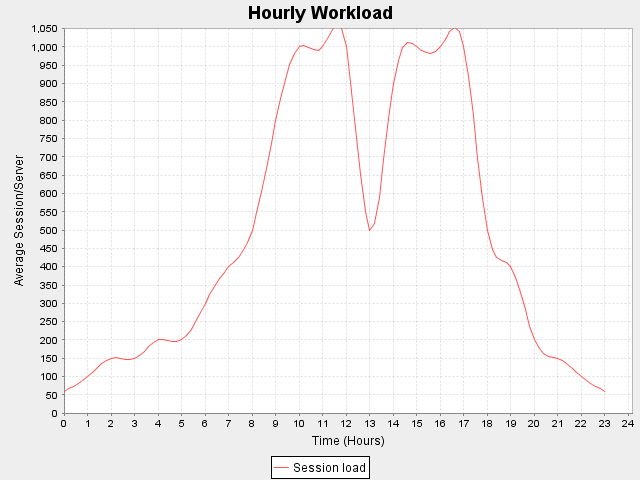
\includegraphics[width=0.75\columnwidth]{results/sim1/sim1-workload.png}
	\caption{Simulation - low workload}
	\label{fig:sim1-workload}
\end{figure}

Figures \ref{fig:sim1-basestats}, \ref{fig:sim1-antSimplestats} and \ref{fig:sim1-antHHstats} show the statistical results for the simulation runs. The results are averaged per hour and across the 5 runs for each auto-scaling algorithm. The graphs include average CPU usage as well as average number of sessions per server and average provisioned servers. Looking at the three graphs, it can be seen that the simple ant auto scaling algorithm obtains better CPU utilization than the simple auto scaling approach, and better than the house hunting algorithm also. At the same time, the simple ant auto scaling algorithm achieves this, while maintaining the server count more stable than the simple auto scaling algorithm.

\begin{figure}
	\centering
		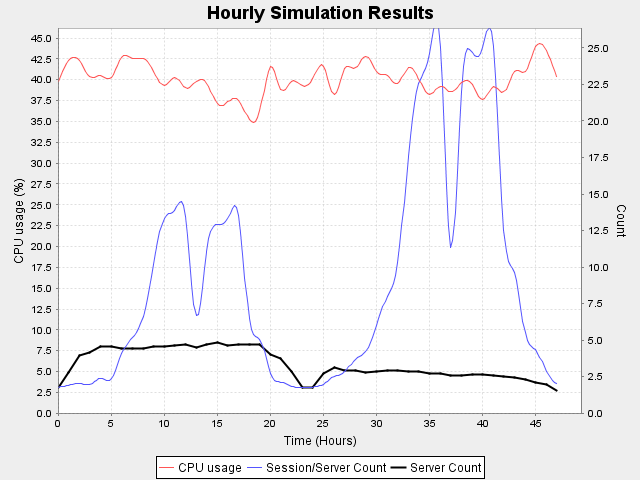
\includegraphics[width=0.75\columnwidth]{results/sim1/sim1-basestats.png}
	\caption{Simulation - Simple autoscaling}
	\label{fig:sim1-basestats}
\end{figure}

\begin{figure}
	\centering
		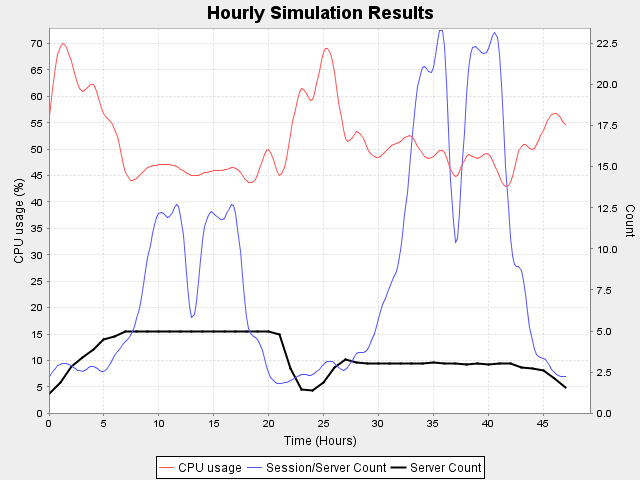
\includegraphics[width=0.75\columnwidth]{results/sim1/sim1-antSimplestats.png}
	\caption{Simulation - Simple ant autoscaling}
	\label{fig:sim1-antSimplestats}
\end{figure}

\begin{figure}
	\centering
		\includegraphics[width=0.75\columnwidth]{results/sim1/sim1-antHHstats.png}
	\caption{Simulation - House hunting ant autoscaling}
	\label{fig:sim1-antHHstats}
\end{figure}

Similar results can be seen in Table \ref{table:sim1} which summarizes the tests. The simple scaling algorithm takes a lot more scale up and scale down actions than the two ant based algorithms. This is because as soon as the average utilization breaches the thresholds an action must be taken, while for the ant algorithms the detection is not triggered by a single drop or spike in utilization. At the same time, the simple ant scaling algorithm has a much shorter time when the cloud is over provisioned (too many servers for the load) compared to the simple scaling algorithm, and longer periods when the cloud is under high usage with over 90\% and 95\% CPU usage. The house hunting algorithm performs worse than the simple ant algorithm for this test, as it tends to over provision the cloud when a breach is predicted by adding too many servers. This can be seen, as it has higher scale up/down counts and also higher over provisioned times.

\begin{table}
\caption{Low workload simulation results}
\label{table:sim1}
\begin{tabu} to\linewidth{|X[c]|X[c]|X[c]|X[c]|X[c]|X[c]|X[c]|X[c]|}
\everyrow{\hline}
\hline
Scaling Algorithm & Scale Up Count & Scale Down Count & Over Provisioned - 10\% (s) & Over Provisioned - 20\% (s) & High usage - 95\% (s) & High usage - 90\% (s) \\
\taburowcolors 2{Gray!20..LimeGreen!50}
Simple scaling & 755 & 762 & 12 & 163 & 3 & 8 \\
Simple ant scaling & 128 & 132 & 9 & 53 & 50 & 79 \\
House hunting scaling & 223 & 339 & 101 & 377 & 37 & 64 \\
\end{tabu}
\end{table}

\subsection{High workload, high number of VMs}

\begin{figure}
	\centering
		\includegraphics[width=0.75\columnwidth]{results/sim2/sim2-workload.png}
	\caption{Simulation - low workload}
	\label{fig:sim2-workload}
\end{figure}

\begin{figure}
	\centering
		\includegraphics[width=0.75\columnwidth]{results/sim2/sim2-basestats.png}
	\caption{Simulation - Simple autoscaling}
	\label{fig:sim2-basestats}
\end{figure}

\begin{figure}
	\centering
		\includegraphics[width=0.75\columnwidth]{results/sim2/sim2-antSimplestats.png}
	\caption{Simulation - Simple ant autoscaling}
	\label{fig:sim2-antSimplestats}
\end{figure}

\begin{figure}
	\centering
		\includegraphics[width=0.75\columnwidth]{results/sim2/sim2-antHHstats.png}
	\caption{Simulation - House hunting ant autoscaling}
	\label{fig:sim2-antHHstats}
\end{figure}

\subsection{Very high workload, very high number of VMs}

\begin{figure}
	\centering
		\includegraphics[width=0.75\columnwidth]{results/sim3/sim3-workload.png}
	\caption{Simulation - low workload}
	\label{fig:sim3-workload}
\end{figure}

\begin{figure}
	\centering
		\includegraphics[width=0.75\columnwidth]{results/sim3/sim3-basestats.png}
	\caption{Simulation - Simple autoscaling}
	\label{fig:sim3-basestats}
\end{figure}

\begin{figure}
	\centering
		\includegraphics[width=0.75\columnwidth]{results/sim3/sim3-antSimplestats.png}
	\caption{Simulation - Simple ant autoscaling}
	\label{fig:sim3-antSimplestats}
\end{figure}

\begin{figure}
	\centering
		\includegraphics[width=0.75\columnwidth]{results/sim3/sim3-antHHstats.png}
	\caption{Simulation - House hunting ant autoscaling}
	\label{fig:sim3-antHHstats}
\end{figure}

\section{Self-organizing self-optimization test conclusions}

The performance tests show that the system behaves as desired and that the ACO algorithm properly detects a breach of SLA when the cloud is under loaded or over loaded while the house hunting algorithm can determine the number of servers added or removed. Due to the randomness which exists inside the house hunting algorithm it is possible to overshoot or undershoot the correct number of servers, however this is corrected quickly after another SLA breach is detected.
